%%%%%%%%%%%%%%%%%%%%%%%%%%%%%%%Section 4%%%%%%%%%%%%%%%%%%%%%%%%%%%%%%%%%%% 

\section{Multiple Linear Regression}\label{sec:MLR}
In the previous sections, we considered a simple scenario where a single, categorical, explanatory variable (Treatment $A$ vs.\@ Treatment $B$) was used to model a desired response variable (score $y$). \par Real-world data is, of course, much more intricate and complex, typically consisting of multiple response variables, with multiple quantitative and categorical/qualitative explanatory features. \newl In this section, we will review how to handle such cases.
\begin{figure*}[t]
\centering
  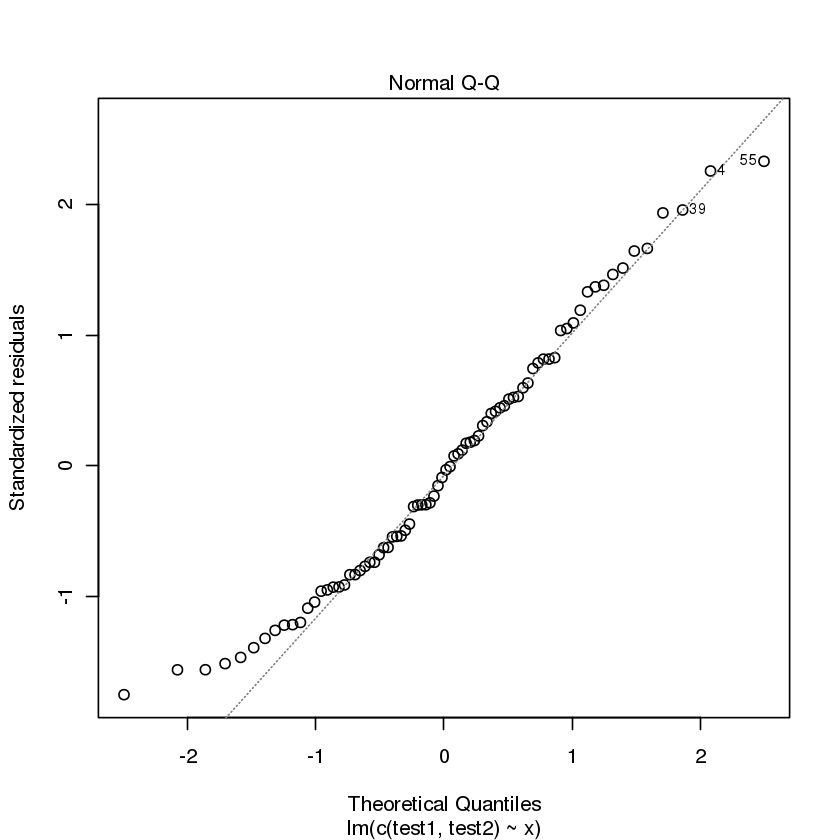
\includegraphics[width=0.475\linewidth]{Images/testA3.png} \quad  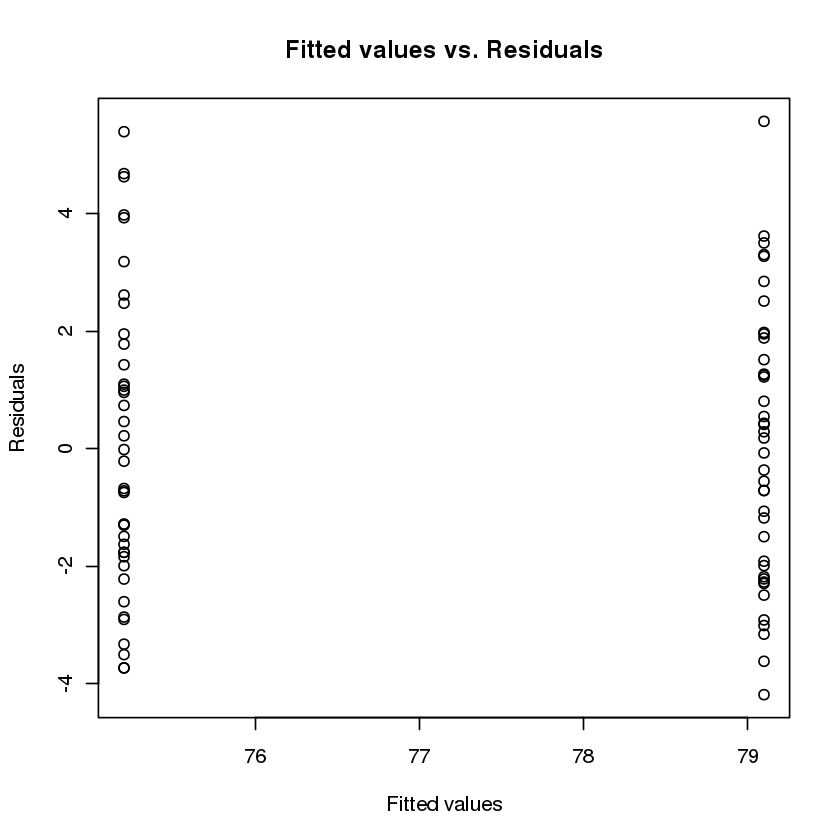
\includegraphics[width=0.475\linewidth]{Images/testA4.png}
  \caption{\small On the left: normal QQ-plot for the two-treatment teaching model (standardised residuals); note the moderate (but acceptable) departure in the lower tail. On the right: diagnostic check for constant variance in the two-treatment teaching model. The spread is fairly similar; we can safely assume constant variance (as well as equal variance across treatment groups).}
  \label{fig:testA3}
\end{figure*}
 \begin{table*}[!t]
         \centering
         \begin{tabular}{c c c c c}
         \hline
        \textbf{Source} & \textbf{Sum of Squares} & \textbf{d.f.} & \textbf{Mean Square} & $\mathbf{F_{0}}$ \\
         \hline
         Regression & $\text{SS}_{\textrm{reg}}$ & $p-1$ & $\text{MS}_{\textrm{reg}}=\text{SS}_{\textrm{reg}}/(p-1)$ & $\text{MS}_{\textrm{reg}}/\text{MS}_{\textrm{e}}$\\
         Error & $\text{SS}_{\textrm{e}}$ & $N-p$ & $\text{MS}_{\textrm{e}}=\text{SS}_{\textrm{e}}/(N-p)$ \\
         Total & $\text{SS}_{\textrm{tot}}$ & $N-1$\\
        \hline
         \end{tabular}
         \caption[\small ANOVA table for first-order multiple regression]{\small ANOVA table for first-order multiple regression model (\ref{eq:MLR}); with $p$ explanatory variables and $N$ observations. }
         \label{tab:SA4}\hrule
     \end{table*}
\subsection{Multiple Linear Regression in Matrix Form}
Throughout, we suppose that the dataset consists of $N$ observations with a single response output $Y$ and $p$ explanatory variables $X_1,\ldots,X_p$. The \textbf{first-order linear model} describing this scenario can be represented in matrix from by 
\begin{equation}\label{eq:MLR}
    \bm{y}=\bm{X\beta}+\bm{\varepsilon},
\end{equation}
where the vectors $\bm{y}=[y_{1},\cdots,y_{N}]^{\!\top}$, $\bm{\beta}=[\beta_{0},\cdots,\beta_{p}]^{\!\top}$, and $\bm{\varepsilon}=[\varepsilon_{1},\cdots,\varepsilon_{N}]^{\!\top}$ are the \textbf{response vector},  the \textbf{coefficient vector}, and  the \textbf{error vector}, respectively, and 
\begin{gather*}
 \bm{X} =  
    \begin{bmatrix}
    1 & x_{1,1} & \cdots & x_{1,p}\\
    \vdots & \vdots & \ddots & \vdots\\
    1 & x_{N,1} & \cdots & x_{N,p}\\
    \end{bmatrix}  
\end{gather*}
is the \textbf{design matrix}, with $\bm{\varepsilon}\sim N(\bm{0}, \sigma^{2}\bm{I}_n)$, where $\bm{I}_n$ is the $N \times N$ \textbf{identity matrix}. 
 
\subsection{Qualitative Explanatory Variables}
Some say that the colour of a vehicle is part of the assessment for car insurance premiums. Such a variable is \textbf{qualitative} (nominal, in fact) in nature, as there is no reasonable way to order colours for insurance purposes. \par If we want to incorporate this feature in an insurance premium model taking into account $k$ possible colour choices (red , black , $\ldots$ , green , yellow), then we need $k-1$ dummy variables $X_1,\ldots,X_{k-1}$ defined according to  
\begin{align*}
    X_{1} &= 
    \begin{cases}
    1 & \text{if red}\\
    0 & \text{otherwise}
    \end{cases}
 \cdots \quad 
    X_{k-1} = 
    \begin{cases}
    1 & \text{if green}\\
    0 & \text{otherwise}
    \end{cases}
\end{align*}
With \textbf{ordinal variables} (e.g., \textit{on scale of 1 to 5, how likely are you to buy a new phone this year?}), we may choose to have 4 dummy variables as above, or a single continuous variable. \newpage\noindent While the latter approach saves 4 degrees of freedom, we are imposing an assumption that equal spacings on the ordinal axis have an equal impact on the outcome, which may not be the case -- if it isn't so, it might be preferable to use dummy variables.

        
\subsection{Overall Significance of the Model}
For the model presented in (\ref{eq:MLR}), \textbf{ordinary least square} (OLS) estimation yields \textbf{fitted values} $$\bm{\hat{y}}=\bm{X\hat{\beta}}=\bm{X}(\bm{XX}^{\!\top})^{-1}\bm{X}^{\!\top}\bm{y}$$ and residuals $$\bm{e}=\bm{y}-\bm{\hat{y}}=(\bm{I}-\bm{X}(\bm{XX}^{\!\top})^{-1}\bm{X}^{\!\top})\bm{y}.$$ The ANOVA table has the same form as Table~\ref{tab:SA2}, although the sums of squares will be different: \begin{align*}
   \text{SS}_{\textrm{tot}}&=\|\bm{y}-\bar{y}\bm{1}\|^2=\sum_{i}(y_{i}-\bar{y})^{2}=\sum_{i}(y_{i}-\hat{y}_i+\hat{y}_i-\bar{y})^{2}\\
    &=\sum_{i}(y_i-\hat{y}_{i})^{2}+\sum_{i}(\hat{y}_{i}-\bar{y})^2=\|\bm{y}-\bm{\hat{y}}\|^2+\|\bm{\hat{y}}-\bar{y}\bm{1}\|^2\\&=\text{SS}_{\textrm{reg}}+\text{SS}_{\textrm{e}}
\end{align*}
(see Table~\ref{tab:SA4}).\newpage\noindent It is used in testing $$H_{0}: \beta_{1} = \cdots = \beta_{p}=0\quad\mbox{against}\quad H_{1}: \beta_{i} \neq 0 \text{ for some  } i.$$ If the test statistic $F_{0}$ is \textbf{significant}, it does not necessarily imply that all the independent variables $X_1, \ldots, X_p$ are useful in predicting $y$, only that at least one of them is. \par We can examine significance of the $\beta$ coefficients individually (using a $t$-test), or multiple coefficients simultaneously (e.g., by building \textbf{Bonferroni simultaneous confidence interval}). Choosing the best subset of the model will be discussed in the next section.

\subsection{Model Adequacy Checks} There are some rare examples for which OLS does not yield a unique solution; but in the vast majority of instances, the data can be fitted to the model. How can we tell if the model is \textbf{adequate} to the situation at hand? 
\begin{itemize}
\item \textbf{Assumptions on Residuals} -- we cannot emphasise enough that \textbf{statistical significance} (i.e. when $F_0$ is in the critical region) \textbf{does not mean that the model is necessarily valid}; the conclusion only follows once the model has been determined to be an \textbf{adequate} fit for the data. A normal-QQ plot can help verify the assumption of normality, for instance, while the assumptions of independence and constant variance can be tested using scatterplots of fitted values against residuals.

\item \textbf{Outliers and Influential Points} -- in addition, \textbf{outliers} and \textbf{influential points} could affect the fitted values. While it is typically easier to classify some observations as outliers, influential points can distort the regression line significantly. Figure \ref{fig:testA5} shows the clear impact of an influential point. Outliers and influential points should be studied carefully, as there are a number of possible mechanisms that can account for their presence; it may be that these anomalies are due to data entry error, in which case we may try to correct/impute with a reasonable alternative, if possible. It may be the case that these unusual observations are worth studying on their own merit.

\begin{figure}[!t]
\centering
  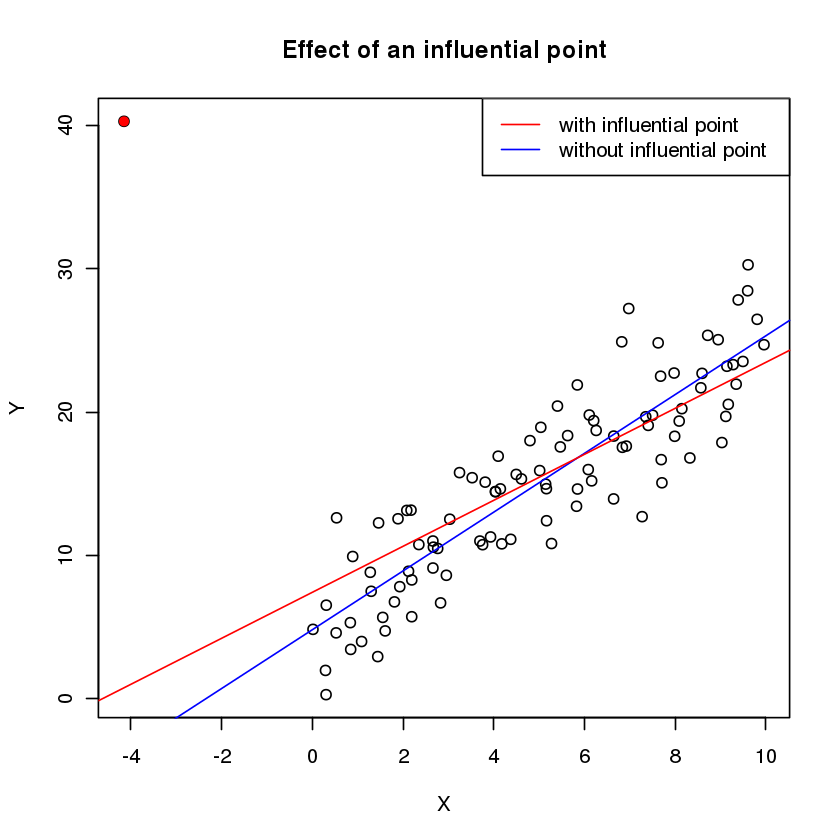
\includegraphics[width=\linewidth]{Images/testA5.png}
  \caption[\small Illustrative example of the effect of an influential point]{\small Illustrative example of the effect of an influential point. The red dot in the top left corner is an influential point -- the slope of the  regression line when it is included in the data (red) is quite different from the slope when it is not (blue).}
  \label{fig:testA5}\hrule
\end{figure}

\item \textbf{Multicollinearity} and \textbf{Variance Inflation Factor} (VIF) -- last but not least, it is important to take a look at the scatterplot matrix and the correlation matrix of the explanatory variables to detect \textbf{multicollinearity}. While it is hoped that the explanatory variables have some relationship with the response variable (otherwise any model is bound to be fruitless), high correlations and/or dependencies among the explanatory variables is contra-indicated as it introduces instability in the estimates of the regression coefficients are unstable. We can formally test for presence of multicollinearity using \textbf{variance inflation factors} (VIF); in its presence, data reduction and data transformation strategies might need to be implemented. 
\end{itemize}


